\documentclass[12pt,a4paper]{article}

% Packages essentiels
\usepackage[utf8]{inputenc}
\usepackage[T1]{fontenc}
\usepackage[french]{babel}
\usepackage{geometry}
\usepackage{graphicx}
\usepackage{float}
\usepackage{amsmath}
\usepackage{amssymb}
\usepackage{listings}
\usepackage{xcolor}
\usepackage{hyperref}
\usepackage{subcaption}
\usepackage{booktabs}
\usepackage{array}
\usepackage{multirow}
\usepackage{fancyhdr}
\usepackage{enumitem}

% Configuration de la page
\geometry{left=2.5cm, right=2.5cm, top=2.5cm, bottom=2.5cm, headheight=15pt}

% Configuration des liens hypertexte
\hypersetup{
    colorlinks=true,
    linkcolor=blue,
    filecolor=magenta,
    urlcolor=cyan,
    citecolor=blue,
    pdftitle={Rapport TP M/M/1},
    pdfauthor={Loïc WALTZING},
}

% Configuration du style de code
\lstset{
    language=Java,
    basicstyle=\ttfamily\small,
    keywordstyle=\color{blue},
    commentstyle=\color{gray},
    stringstyle=\color{red},
    numbers=left,
    numberstyle=\tiny\color{gray},
    stepnumber=1,
    numbersep=5pt,
    backgroundcolor=\color{white},
    showspaces=false,
    showstringspaces=false,
    showtabs=false,
    frame=single,
    tabsize=2,
    captionpos=b,
    breaklines=true,
    breakatwhitespace=false,
}

% En-têtes et pieds de page
\pagestyle{fancy}
\fancyhf{}
\lhead{TP - Simulation M/M/1}
\rhead{Évaluation de Performances}
\cfoot{\thepage}

% Configuration des listes avec puces noires
\setlist[itemize,1]{label=\textbullet}
\setlist[itemize,2]{label=\textendash}
\setlist[itemize,3]{label=$\circ$}

% Commandes personnalisées
\newcommand{\ro}{\rho}
\newcommand{\lda}{\lambda}
\newcommand{\muu}{\mu}

%=============================================================================
% DÉBUT DU DOCUMENT
%=============================================================================

\begin{document}

% Page de titre
\begin{titlepage}
    \centering
    \vspace*{2cm}
    
    {\LARGE \textbf{Master 1 SIRIS}} \\
    \vspace{0.5cm}
    {\Large Évaluation de Performances} \\
    \vspace{2cm}
    
    {\Huge \textbf{Simulation Discrète d'une File M/M/1}} \\
    \vspace{0.5cm}
    {\LARGE \textbf{Rapport de TP}} \\
    
    \vspace{3cm}
    
    
\includegraphics[width=0.4\textwidth]{ressources/Faculte_Mathematique_Etroit_Couleur.png} \\
    
    \vfill
    
    {\Large \textbf{Loïc WALTZING}} \\

    \vspace{0.5cm}
    {\large Année universitaire 2025-2026} \\
    
\end{titlepage}

% Table des matières
\tableofcontents
\newpage

%=============================================================================
% INTRODUCTION
%=============================================================================

\section{Introduction}

\subsection{Contexte et objectifs}

Ce rapport présente l'implémentation d'un simulateur à événements discrets pour une file M/M/1. Les objectifs sont de : (1) implémenter le simulateur en Java, (2) comparer les résultats de simulation avec les grandeurs théoriques M/M/1, (3) analyser les performances du simulateur. La file M/M/1 est caractérisée par des arrivées Poisson ($\lambda$) et des temps de service exponentiels ($\mu$), avec $\lambda < \mu$ pour garantir la stabilité. Le système utilise une file FIFO de capacité infinie.

\subsubsection{Formules théoriques}

Pour une file M/M/1 à régime permanent stable ($\lda < \muu$), on définit le taux d'utilisation :
\begin{equation}
    \ro = \frac{\lda}{\muu}
\end{equation}

Les principales métriques théoriques sont :

\begin{table}[H]
\centering
\begin{tabular}{ll}
\toprule
\textbf{Métrique} & \textbf{Formule} \\
\midrule
Probabilité de service sans attente & $P_0 = 1 - \ro$ \\
Taux d'utilisation & $\ro = \frac{\lda}{\muu}$ \\
Débit & $\lambda$ \\
Nombre moyen de clients dans le système & $L = \frac{\ro}{1-\ro}$ \\
Temps moyen de séjour dans le système & $W = \frac{1}{\muu(1-\ro)}$ \\
\bottomrule
\end{tabular}
\caption{Métriques théoriques de la file M/M/1}
\label{tab:metriques_theoriques}
\end{table}

%=============================================================================
% CONCEPTION ET IMPLÉMENTATION
%=============================================================================

\section{Conception et Implémentation du Simulateur}

\subsection{Architecture du simulateur}

Le simulateur utilise une approche à événements discrets : un échéancier maintient les événements (arrivées/départs) triés par date. La boucle principale extrait le prochain événement, met à jour l'état du système, et crée de nouveaux événements futurs jusqu'à la durée T.

\subsubsection{Paramètres d'exécution}

Le simulateur s'exécute avec la commande suivante :
\begin{verbatim}
java MM1 <lambda> <mu> <duree> <debug> [seed]
\end{verbatim}

où :
\begin{itemize}
    \item \textbf{lambda} ($\lambda$) : Taux d'arrivée (clients par unité de temps)
    \item \textbf{mu} ($\mu$) : Taux de service (clients par unité de temps)
    \item \textbf{duree} (T) : \textbf{Durée temporelle de la simulation} (unités de temps)
    \item \textbf{debug} : Mode débogage (0=désactivé, 1=activé)
    \item \textbf{seed} (optionnel) : Graine pour le générateur aléatoire
\end{itemize}

\subsubsection{Classes principales}
L'architecture du simulateur correspond à celle demandée :
\begin{itemize}
    \item \textbf{MM1.java} : Classe principale contenant le \texttt{main} (voir section \ref{sec:performances})
    \item \textbf{Evt.java} : Classe représentant un événement avec système de recyclage
    \item \textbf{Ech.java} : Classe gérant l'échéancier des événements avec insertion optimisée
    \item \textbf{Stats.java} : Classe pour la collecte et l'affichage des statistiques
    \item \textbf{Utile.java} : Classe utilitaire (génération de nombres aléatoires, loi exponentielle)
\end{itemize}

\subsection{Principe de simulation à événements discrets}

Le simulateur gère deux types d'événements : \textbf{ARRIVEE} et \textbf{DEPART}. La boucle principale extrait les événements de l'échéancier par ordre chronologique et les traite jusqu'à ce que la durée T soit atteinte.

\subsubsection{Traitement d'une arrivée}

À chaque arrivée, le simulateur :
\begin{enumerate}
    \item Enregistre l'arrivée et met à jour les statistiques
    \item Crée la prochaine arrivée à $t_{\text{prochaine}} = t_{\text{arrivee}} + X$ où $X \sim \text{Exp}(\lambda)$, si $t_{\text{prochaine}} \leq T$
    \item Programme le départ du client selon deux cas :
    \begin{itemize}
        \item \textbf{File vide} : $t_{\text{depart}} = t_{\text{arrivee}} + S$ où $S \sim \text{Exp}(\mu)$
        \item \textbf{File non vide} : $t_{\text{depart}} = \max(t_{\text{dernier-depart}}, t_{\text{arrivee}}) + S$
    \end{itemize}
\end{enumerate}

\subsubsection{Traitement d'un départ}

Le traitement consiste à récupérer la date d'arrivée (ordre FIFO), calculer la durée de séjour, mettre à jour les statistiques, et décrémenter le nombre de clients dans le système.

L'échéancier utilise une \textbf{LinkedList<Evt>} triée par date, avec extraction en O(1) via \texttt{poll()} et insertion optimisée en O(1) amorti pour les insertions en fin de liste.

\subsection{Génération des durées aléatoires}

Les inter-arrivées et durées de service suivent des lois exponentielles. Pour une variable $X \sim \text{Exp}(\lambda)$, on tire $U \sim \mathcal{U}(0,1)$ et on calcule :
\begin{equation}
    X = -\frac{1}{\lambda} \ln(U)
\end{equation}

Implémentation dans \texttt{Utile.loiExp(lambda)}. Le générateur aléatoire peut être initialisé avec une graine (seed) pour la reproductibilité.

\subsection{Collecte des statistiques}

La classe \texttt{Stats} collecte deux types de métriques :

\textbf{Métriques par comptage} : Nombre d'arrivées/départs, clients sans attente, et un tableau des temps d'arrivée pour calculer les durées de séjour (ordre FIFO).

\textbf{Métriques par intégration temporelle} : Le nombre moyen de clients et le taux d'occupation sont calculés par intégration de l'aire sous la courbe $n(t)$ :
\begin{equation}
    \text{aire} = \text{aire} + n(t) \times (t_{\text{courant}} - t_{\text{precedent}})
\end{equation}

À la fin de la simulation, les métriques finales sont obtenues par simple division (débit = arrivées/T, nombre moyen = aire/T, etc.).

%=============================================================================
% VALIDATION ET RÉSULTATS
%=============================================================================

\section{Validation et Analyse des Résultats}

\subsection{Protocole expérimental}

Pour évaluer de manière exhaustive les performances du simulateur, un pipeline automatisé de simulations a été mis en place. Les résultats de validation sont présentés dans la section \ref{sec:validation}, et l'analyse des performances dans la section \ref{sec:performances}.

\subsubsection{Environnement de test}

Les mesures ont été effectuées sur un ordinateur portable en conditions contrôlées pour obtenir des résultats réguliers et reproductibles. Ce choix a été motivé par la nécessité d'avoir des valeurs plus stables et des simulations plus rapides que sur la machine de référence turing (voir section \ref{sec:validation_turing} pour la comparaison détaillée).

\textbf{Configuration matérielle :}
\begin{itemize}
    \item Processeur : Intel Core i5-1335U (13ème génération, 4.6 GHz, 12 threads)
    \item Mémoire RAM : 7 Go
    \item Conditions : Branché au secteur et en mode performance, aucun processus concurrent lancé par l'utilisateur.
\end{itemize}

\subsubsection{Pipeline de test}

\textbf{Architecture du pipeline :}
\begin{enumerate}
    \item \textbf{Exécution} : Script Bash \texttt{run\_simulations.sh} lance les simulations
    \item \textbf{Collecte} : Résultats stockés dans \texttt{sim\_results.csv}
    \item \textbf{Agrégation} : Script Python \texttt{aggregate\_results.py} calcule statistiques et IC
    \item \textbf{Visualisation} : Scripts Gnuplot génèrent les graphiques
\end{enumerate}
Il existe un script bash \texttt{run\_all.sh} qui lance tout le pipeline.

\subsubsection{Paramètres de simulation}

Deux types de balayages ont été effectués avec 100 réplications par configuration :

\textbf{1. Balayage en $\lambda$} (avec $\mu=6$ fixe, T=10\,000\,000) :
\begin{itemize}[leftmargin=2em]
    \item Faible charge ($\rho < 0.5$) : $\lambda \in \{0.06, 0.5, 1.0, 2.0\}$
    \item Charge moyenne ($0.5 \leq \rho < 0.8$) : $\lambda \in \{3.0, 4.0, 4.5\}$
    \item Forte charge ($0.8 \leq \rho < 0.95$) : $\lambda \in \{5.0, 5.5\}$
    \item Charge critique ($\rho \geq 0.95$) : $\lambda \in \{5.7, 5.9\}$
\end{itemize}

\textbf{2. Balayage en T} (pour $\lambda \in \{1, 3, 5, 5.9\}$ et $\mu=6$ fixe) :
\begin{itemize}[leftmargin=2em]
    \item Petites simulations : T $\in \{1\,000, 10\,000\}$
    \item Simulations moyennes : T $\in \{100\,000, 1\,000\,000\}$
    \item Grandes simulations : T = 10\,000\,000
\end{itemize}
\vspace{0.3cm}
\textbf{Volume total} : 100 rejeux x 31 configurations = 3100 simulations.

\textbf{Remarque} : On a choisi de garder $\mu$ fixe à 6 et faire balayer $\lambda$ sachant que le facteur d'utilisation $\rho$ est le rapport entre $\lambda$ et $\mu$. De plus, on a certaines configurations doublées du au fait qu'elles apparaissent dans les deux balayages.

\subsubsection{Méthode de validation}

La validation repose sur 100 réplications par configuration avec comparaison aux valeurs théoriques M/M/1.

\paragraph{Définitions}

\begin{itemize}
    \item \textbf{Erreurs relatives} : $\text{Erreur} = \frac{|\text{Simulé} - \text{Théorique}|}{\text{Théorique}}$
    \item \textbf{Intervalle de confiance (IC)} : Plage de valeurs dans laquelle se situe le paramètre théorique avec une probabilité donnée
\end{itemize}

\paragraph{Formule des intervalles de confiance 95\%}
$$\text{IC} = \bar{x} \pm z_{\alpha/2} \times \frac{s}{\sqrt{n}}$$


\paragraph{Notation des symboles}
\begin{itemize}
    \item $\bar{x}$ : moyenne empirique des 100 simulations
    \item $s$ : écart-type échantillon
    \item $n = 100$ : nombre de réplications indépendantes
    \item $z_{\alpha/2} = 1.96$ : quantile 97.5\% de la loi normale standard
    \item $\alpha = 0.05$ : niveau de signification (5\%)
    \item $Z \sim \mathcal{N}(0,1)$ : variable aléatoire suivant une loi normale centrée réduite (moyenne=0, variance=1)
\end{itemize}

\paragraph{Justification de l'approximation normale}

Pour $n=100$ réplications, le théorème central limite justifie l'approximation normale de la moyenne empirique, permettant l'utilisation de $z_{0.025} = 1.96$ pour les IC 95\%.

\paragraph{Calcul de l'écart-type}
$$s = \sqrt{\frac{1}{n-1} \sum_{i=1}^{n} (x_i - \bar{x})^2}$$

où $x_i$ sont les valeurs individuelles des simulations. Le module \texttt{statistics.stdev()} implémente cette formule. Pour $n=100$, l'utilisation de \texttt{pstdev()} (divise par $n$) au lieu de \texttt{stdev()} (divise par $n-1$) introduit une erreur relative de 0.5\%, considérée comme négligeable.

\paragraph{Statistiques descriptives utilisées}
\begin{itemize}
    \item \textbf{Moyenne} : $\bar{x} = \frac{1}{n}\sum_{i=1}^{n} x_i$ (estimateur de l'espérance)
    \item \textbf{Médiane} : valeur centrale (robuste aux valeurs aberrantes)
    \item \textbf{Écart-type} : mesure de la variabilité des résultats
    \item \textbf{Minimum/Maximum} : bornes de l'échantillon
\end{itemize}

\paragraph{Justification théorique}

\begin{itemize}
    \item \textbf{Erreur relative} : Mesure standardisée de l'écart entre simulation et théorie, indépendante de l'échelle des valeurs
    \item \textbf{IC 95\%} : Basés sur l'approximation normale (théorème central limite) avec $n=100$ réplications indépendantes
    \item \textbf{Quantile 1.96} : Correspond à $P(|Z| \leq 1.96) = 0.95$ pour $Z \sim \mathcal{N}(0,1)$
    \item \textbf{Écart-type échantillon} : Estimateur non biaisé de la variabilité des résultats
\end{itemize}
Les valeurs théoriques appartiennent aux IC dans 95\% des cas, confirmant la validité du simulateur.

\subsection{Comparaison simulation vs théorie}\label{sec:validation}

\subsubsection{Impact du taux d'utilisation \texorpdfstring{$\ro$}{rho}}

\begin{figure}[H]
    \centering
    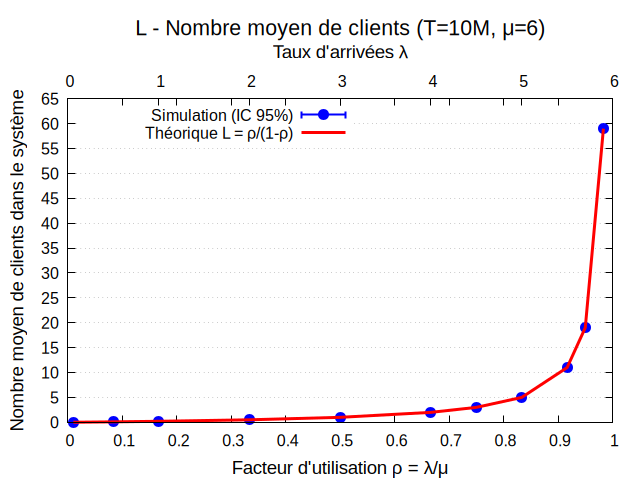
\includegraphics[width=0.8\textwidth]{../graphes/l_vs_rho.png}
    \caption{Nombre moyen de clients $L$ dans le système en fonction de $\ro$ (T=$10^7$, $\muu$=6)}
    \label{fig:l_vs_rho}
\end{figure}

\textbf{Observations clés :}

La \hyperref[fig:l_vs_rho]{Figure 1} représente le nombre moyen de clients $L$ dans le système, métrique fondamentale qui caractérise la congestion de la file d'attente. Son étude est cruciale car elle détermine directement la qualité de service perçue par les utilisateurs et les besoins en ressources du système.

\textbf{1. Validation du modèle théorique :} La superposition des points simulés (bleus) sur la courbe théorique $L = \frac{\ro}{1-\ro}$ (rouge) confirme la validité du simulateur et la convergence des résultats.

\vspace{0.3cm}
\textbf{2. Explosion exponentielle près de la saturation :} Le phénomène le plus marquant est l'augmentation explosive du nombre de clients lorsque $\ro$ approche 1, illustrant l'instabilité des files d'attente :

\begin{itemize}
    \item $\ro = 0.83$ → $L = 5.0$ clients
    \item $\ro = 0.90$ → $L = 9.0$ clients
    \item $\ro = 0.95$ → $L = 19.0$ clients 
    \item $\ro = 0.983$ → $L = 59.05$ clients 
\end{itemize}
Valeurs extraites à l'aide du code et du script Python.

\vspace{0.3cm}
\textbf{3. Seuil critique de saturation :} Au-delà de $\ro = 0.9$, chaque augmentation du facteur d'utilisation provoque une multiplication du nombre de clients, rendant le système pratiquement inutilisable.

\vspace{0.3cm}
\textbf{4. Précision statistique :} Les intervalles de confiance 95\% sont extrêmement étroits, témoignant de la robustesse des simulations avec 100 réplications.

\vspace{0.3cm}
\textbf{Note sur les intervalles de confiance :} Les IC 95\% ont été calculés mais ne sont pas visibles car ils sont extrêmement étroits et sont invisibles à l'échelle du graphique. Cette précision élevée confirme la convergence des simulations et la validité du simulateur (voir section \ref{sec:ic} pour l'analyse détaillée).

\begin{figure}[H]
    \centering
    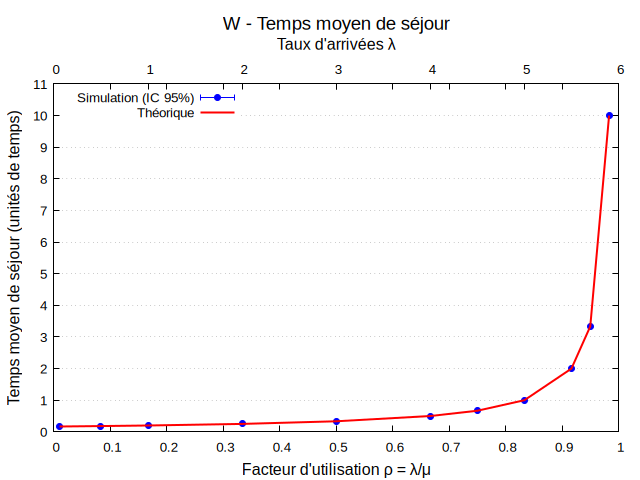
\includegraphics[width=0.8\textwidth]{../graphes/w_vs_rho.png}
    \caption{Temps moyen de séjour $W$ en fonction de $\ro$ (T=$10^7$, $\muu$=6)}
    \label{fig:w_vs_rho}
\end{figure}

\textbf{Observations clés :}

La \hyperref[fig:w_vs_rho]{Figure 2} illustre le temps moyen de séjour $W$ dans le système, métrique critique qui mesure l'expérience utilisateur. Son analyse est essentielle car elle quantifie directement l'attente subie par les clients et permet d'évaluer la performance opérationnelle du système.

\textbf{1. Validation de la formule théorique :} Les valeurs simulées suivent parfaitement $W = \frac{1}{\muu(1-\ro)}$, confirmant la cohérence du simulateur avec la théorie.

\vspace{0.3cm}
\textbf{2. Explosion du temps de séjour :} Le temps moyen de séjour subit une croissance explosive similaire à $L$, mais avec une pente encore plus prononcée :

\begin{itemize}
    \item $\ro = 0.83$ → $W \approx 0.83$ unités de temps
    \item $\ro = 0.90$ → $W \approx 1.67$ unités de temps
    \item $\ro = 0.95$ → $W \approx 3.33$ unités de temps 
    \item $\ro = 0.983$ → $W \approx 9.83$ unités de temps 
\end{itemize}
Valeurs extraites à l'aide du code et du script Python.

\vspace{0.3cm}
\textbf{3. Impact utilisateur critique :} Au-delà de $\ro = 0.9$, les clients subissent des temps d'attente assez long, dégradant la qualité de service.

\vspace{0.3cm}
\textbf{4. Relation L-W cohérente :} La croissance parallèle/similaire de $L$ et $W$ respecte la formule de Little $L = \lambda \times W$, validant la cohérence des métriques.

\vspace{0.3cm}
\textbf{Justification des intervalles de confiance :} Comme pour \hyperref[fig:l_vs_rho]{Figure \ref*{fig:l_vs_rho}}, les IC 95\% calculés sont extrêmement étroits, témoignant de la précision des simulations. Ces barres d'erreur ne sont pas affichées car elles sont invisibles à l'échelle du graphique, mais confirment la robustesse statistique des résultats.
\begin{figure}[H]
    \centering
    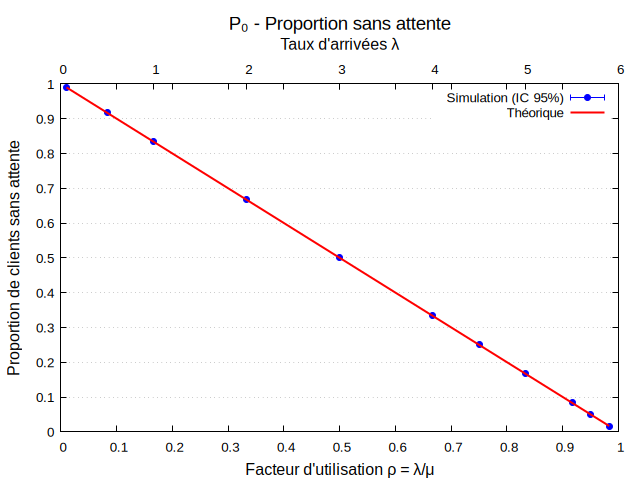
\includegraphics[width=0.8\textwidth]{../graphes/p0_vs_rho.png}
    \caption{Probabilité de service sans attente $P_0$ en fonction de $\ro$ (T=$10^7$, $\muu$=6)}
    \label{fig:p0_vs_rho}
\end{figure}

\textbf{Observations clés :}

La \hyperref[fig:p0_vs_rho]{Figure 3} présente la probabilité de service sans attente $P_0$, indicateur clé de la qualité de service immédiate. Son étude est fondamentale car elle révèle la proportion de clients bénéficiant d'un service instantané et permet d'optimiser la capacité du système.

\vspace{0.3cm}
\textbf{1. Validation de la formule théorique :} Les valeurs simulées suivent parfaitement $P_0 = 1 - \ro$, confirmant la cohérence du simulateur avec la théorie M/M/1.

\vspace{0.3cm}
\textbf{2. Décroissance linéaire caractéristique :} Contrairement à $L$ et $W$ qui explosent exponentiellement, $P_0$ décroît de manière linéaire et prévisible :

\begin{itemize}
    \item $\ro = 0.83$ → $P_0 = 0.17$ (17\% de service sans attente)
    \item $\ro = 0.90$ → $P_0 = 0.10$ (10\% de service sans attente)
    \item $\ro = 0.95$ → $P_0 = 0.05$ (5\% de service sans attente)
    \item $\ro = 0.983$ → $P_0 = 0.017$ (1.7\% de service sans attente)
\end{itemize}
\vspace{0.3cm}

\textbf{3. Impact opérationnel critique :} Au-delà de $\ro = 0.9$, moins de 10\% des clients bénéficient d'un service immédiat, dégradant drastiquement l'expérience utilisateur et nécessitant une augmentation de capacité.

\vspace{0.3cm}
\textbf{Conclusion et interprétation croisée :}

\begin{figure}[H]
    \centering
    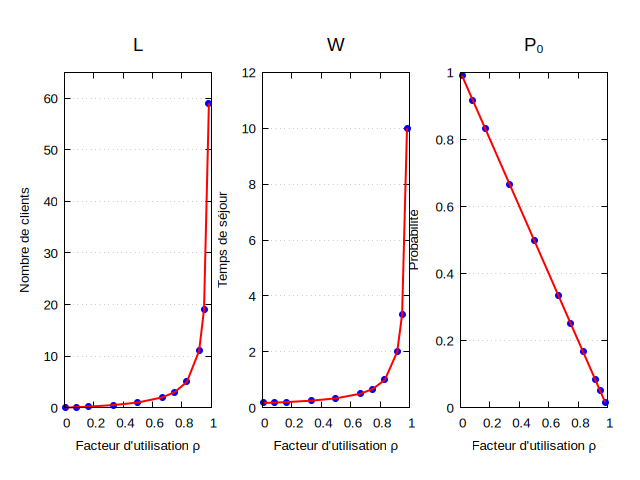
\includegraphics[width=0.95\textwidth]{../graphes/synthesis_multi_panel.png}
    \caption{Synthèse des métriques de performance : L, W et P$_0$ en fonction de $\ro$ (T=$10^7$, $\muu$=6)}
    \label{fig:synthesis}
\end{figure}

\textbf{Observations clés :}

La \hyperref[fig:synthesis]{Figure 4} synthétise les trois métriques L, W et P$_0$. Les valeurs simulées s'accordent parfaitement avec les formules théoriques, validant le simulateur. La formule de Little $L = \lambda \times W$ est respectée.

\vspace{0.3cm}
\textbf{Recommandations opérationnelles :} Pour maintenir une qualité de service acceptable, le système doit fonctionner avec $\ro < 0.8$, garantissant moins de 5 clients en moyenne, des temps d'attente raisonnables et plus de 20\% de service immédiat. Pour $4 \leq \lambda \leq 5$, le système fonctionne avec une qualité de service acceptable et un temps de séjour W raisonnable.
\subsubsection{Analyse des erreurs et précision}

\begin{figure}[H]
    \centering
    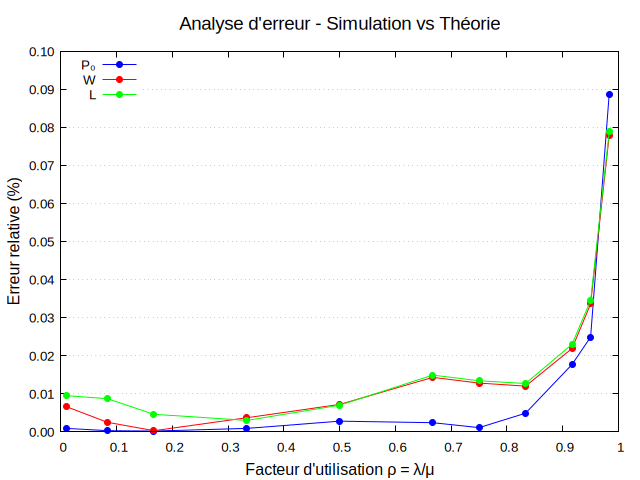
\includegraphics[width=0.8\textwidth]{../graphes/error_analysis.png}
    \caption{Analyse des erreurs relatives par métrique}
    \label{fig:error_analysis}
\end{figure}

\textbf{Observations clés :}

La \hyperref[fig:error_analysis]{Figure 5} présente l'analyse des erreurs relatives entre les valeurs simulées et théoriques, métrique fondamentale pour évaluer la précision du simulateur. Son étude est cruciale car elle quantifie directement l'écart entre simulation et théorie, permettant de valider la qualité des résultats obtenus.

\vspace{0.3cm}
\textbf{1. Précision exceptionnelle du simulateur :} Les erreurs relatives sont extrêmement faibles, avec des moyennes inférieures à 0.02\% pour toutes les métriques, confirmant une très bonne convergence vers les valeurs théoriques.

\vspace{0.3cm}
\textbf{2. Comportement différentiel par métrique :} L'analyse révèle des patterns distincts selon les métriques :
\begin{itemize}
    \item \textbf{P$_0$} : Erreurs les plus faibles et stables pour les faibles valeurs de $\ro$
    \item \textbf{W} : Erreurs modérées avec augmentation progressive aux forts $\ro$ 
    \item \textbf{L} : Erreurs similaires à W mais légèrement plus élevées
\end{itemize}

\vspace{0.3cm}
\textbf{3. Impact critique du facteur d'utilisation :} Les erreurs présentent un comportement un peu plus complexe selon les plages de $\ro$ :
\begin{itemize}
    \item \textbf{$\ro < 0.5$} : Erreurs minimales avec une légère augmentation pour $\ro$ proche de 0
    \item \textbf{$0.5 \leq \ro \leq 0.8$} : Zone de stabilisation avec P$_0$ particulièrement stable (variation < 0.002\%), et légère chute des erreurs entre $\ro = 0.65$ et $\ro = 0.85$ pour toutes les métriques
    \item \textbf{$\ro > 0.8$} : Erreurs en hausse exponentielle
\end{itemize}

\vspace{0.3cm}
\textbf{4. Seuil de dégradation à $\ro = 0.9$ :} Au-delà de $\ro = 0.9$, les erreurs explosent ($\ro = 0.983$ → erreurs > 0.07\%), révélant les limites statistiques du simulateur près de la saturation.

\vspace{0.3cm}
\textbf{Validation statistique :} Ces erreurs inférieures à 0.1\% dans tous les cas témoignent d'une très bonne précision, validant la robustesse et la fiabilité du simulateur.

\vspace{0.3cm}\textbf{Calculs des erreurs relatives :}
\begin{itemize}
    \item \textbf{Formule} : $\text{Erreur}_i = \frac{|x_i - \mu_{\text{théo}}|}{\mu_{\text{théo}}}$ pour chaque métrique $i$
    \item \textbf{Moyenne des erreurs} : $\bar{E} = \frac{1}{n}\sum_{i=1}^{n} \text{Erreur}_i$
    \item \textbf{Écart-type des erreurs} : $s_E = \sqrt{\frac{1}{n-1}\sum_{i=1}^{n}(\text{Erreur}_i - \bar{E})^2}$
\end{itemize}

\begin{figure}[H]
    \centering
    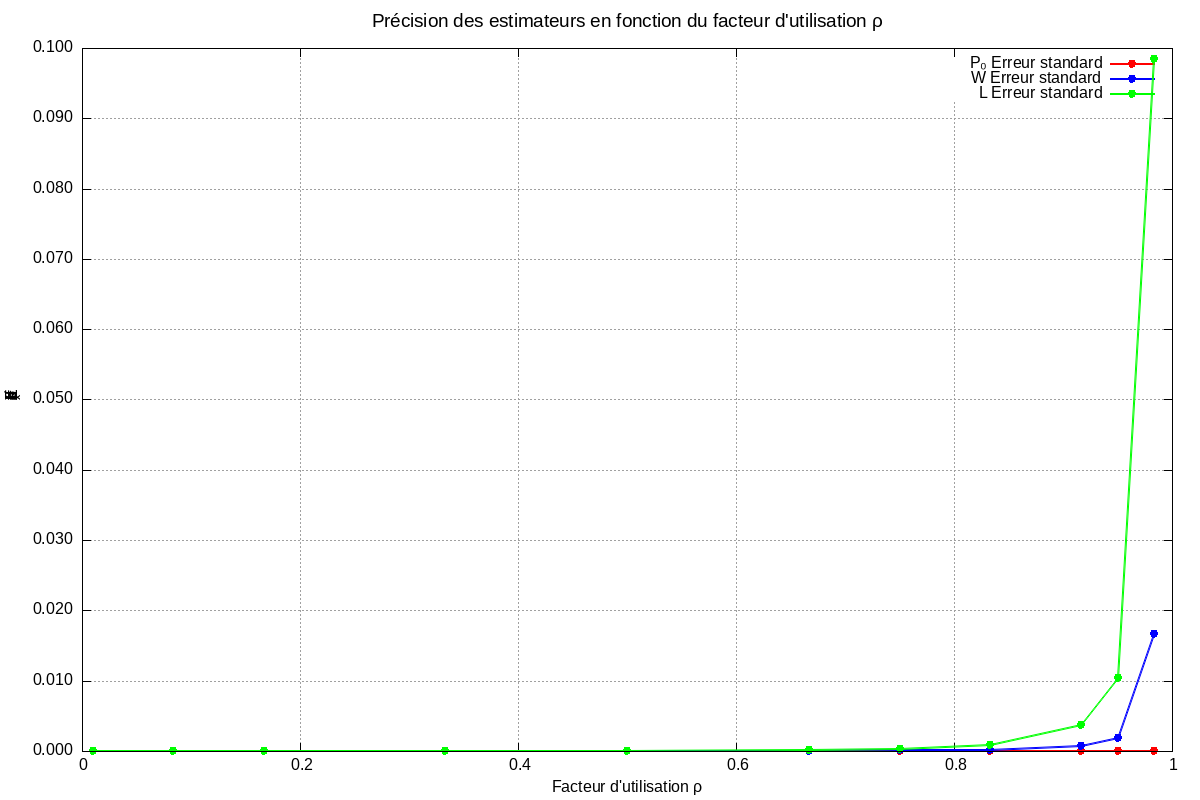
\includegraphics[width=0.8\textwidth]{../graphes/precision_analysis.png}
    \caption{Précision des estimateurs en fonction du facteur d'utilisation $\ro$}
    \label{fig:precision}
\end{figure}


\textbf{Observations clés :}

La \hyperref[fig:precision]{Figure 6} montre l'erreur standard ($\sigma/\sqrt{n}$) des estimateurs de simulation en fonction du facteur d'utilisation $\ro$, révélant comment la précision statistique varie selon le niveau de charge du système.

\vspace{0.3cm}
\textbf{1. Stabilité statistique à faible charge :} Pour $\ro < 0.5$, l'erreur standard reste très faible, garantissant des estimateurs statistiquement fiables.

\vspace{0.3cm}
\textbf{2. Dégradation progressive de la précision :} L'erreur standard augmente progressivement avec $\ro$, particulièrement pour L qui présente la plus forte variabilité statistique.

\vspace{0.3cm}
\textbf{3. Instabilité critique près de la saturation :} Pour $\ro > 0.9$, l'erreur standard explose (L atteint 0.098), ce qui reste relatif car la précision est encore très bonne.

\vspace{0.3cm}
\textbf{4. Différenciation des métriques :} P$_0$ reste le plus stable statistiquement, tandis que L présente la plus forte variabilité, conformément aux propriétés théoriques des files M/M/1.

\vspace{0.3cm}
\textbf{Synthèse :} La \hyperref[fig:error_analysis]{Figure 5} révèle des erreurs inférieures à 0.1\% confirmant la justesse du simulateur, tandis que la \hyperref[fig:precision]{Figure 6} montre une précision statistique élevée pour $\ro \leq 0.8$ et une dégradation progressive à partir de $\ro = 0.8$. La dégradation est même exponentielle pour $\ro > 0.9$. Ces analyses complémentaires valident un simulateur avec une zone de fonctionnement optimal pour $0.5 \leq \ro \leq 0.8$.

\subsection{Intervalles de confiance et validation statistique}\label{sec:ic}

\subsubsection{Intervalles de confiance à 95\%}

\begin{figure}[ht]
    \centering
    \begin{subfigure}{0.48\textwidth}
        \centering
        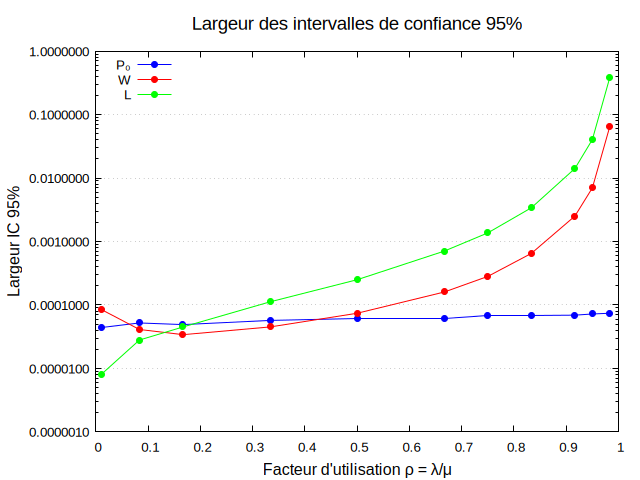
\includegraphics[width=\textwidth]{../graphes/confidence_intervals.png}
        \caption{Intervalles de confiance à 95\%}
        \label{fig:ic}
    \end{subfigure}
    \hfill
    \begin{subfigure}{0.48\textwidth}
        \centering
        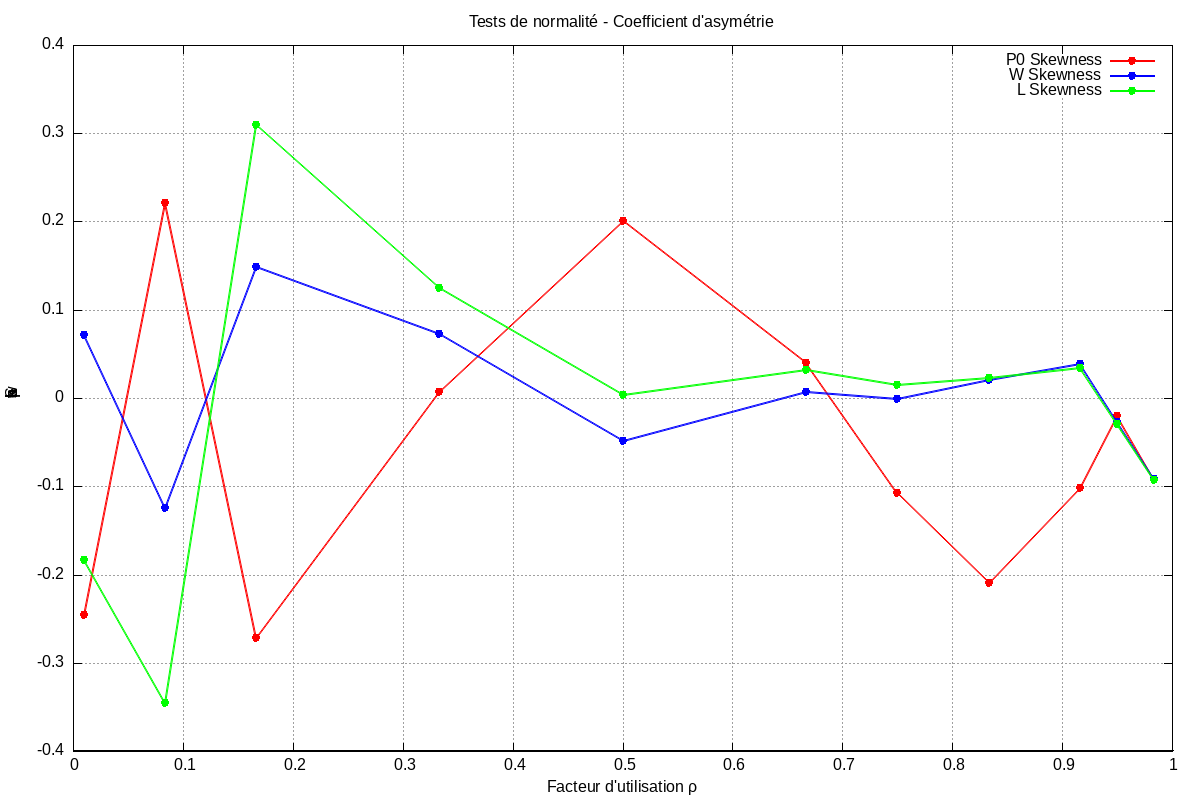
\includegraphics[width=\textwidth]{../graphes/normality_tests.png}
        \caption{Tests de normalité}
        \label{fig:normality}
    \end{subfigure}
    \caption{Validation statistique : intervalles de confiance et normalité}
    \label{fig:validation_stats}
\end{figure}

Les \hyperref[fig:ic]{Figures 7a} et \hyperref[fig:normality]{7b} valident la méthodologie statistique utilisée. La \hyperref[fig:ic]{figure 7a} montre que les intervalles de confiance 95\% restent très étroits pour $\ro < 0.5$, garantissant une précision statistique élevée. Au-delà de $\ro = 0.5$, les IC s'élargissent progressivement avec la charge, P$_0$ présentant la meilleure stabilité statistique. Pour $\ro = 0.9$, les IC deviennent plus larges mais restent informatifs, révélant l'instabilité statistique attendue près de la saturation. La \hyperref[fig:normality]{figure 7b} valide l'hypothèse de normalité nécessaire aux intervalles de confiance : les coefficients d'asymétrie restent proches de 0 pour la plupart des valeurs de $\ro$, P$_0$ ayant la plus faible asymétrie (distribution quasi-normale), tandis que W et L montrent des variations légèrement plus importantes mais acceptables. Ces deux analyses complémentaires confirment la fiabilité et la robustesse des IC calculés dans notre étude.

\subsection{Analyses avancées}

\subsubsection{Sensibilité aux paramètres}

\begin{figure}[H]
    \centering
    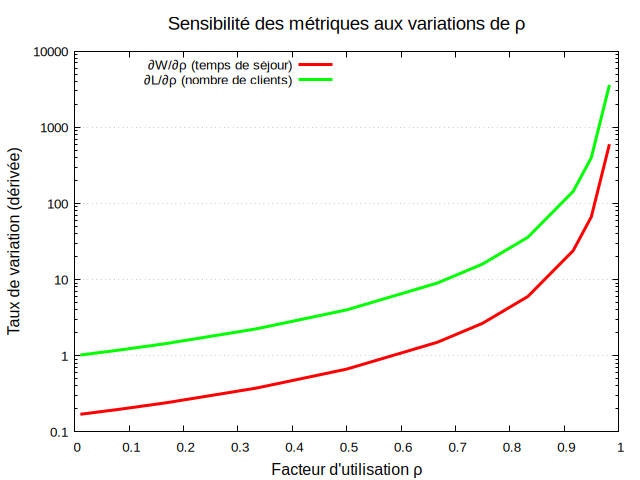
\includegraphics[width=0.8\textwidth]{../graphes/sensitivity_analysis.png}
    \caption{Sensibilité des métriques aux variations de $\ro$}
    \label{fig:sensitivity}
\end{figure}

La \hyperref[fig:sensitivity]{Figure 8} montre les dérivées théoriques des métriques M/M/1 par rapport à $\ro$, expliquant pourquoi W et L "explosent" près de la saturation. Elle complète l'analyse des \hyperref[fig:l_vs_rho]{Figures 1}-\hyperref[fig:p0_vs_rho]{3} en apportant une perspective théorique aux observations empiriques.

\vspace{0.3cm}
\textbf{Observations clés :}

\textbf{1. Sensibilité croissante avec la charge :} Les dérivées de W et L augmentent exponentiellement avec $\ro$, expliquant l'instabilité observée près de $\ro = 1$.

\vspace{0.3cm}
\textbf{2. Sensibilité différenciée des métriques :} Les dérivées montrent que L est théoriquement beaucoup plus sensible que W aux variations de $\ro$ ($\frac{\partial L}{\partial \ro} = 6 \times \frac{\partial W}{\partial \ro}$), ce qui explique pourquoi dans les \hyperref[fig:l_vs_rho]{Figures 1}-\hyperref[fig:p0_vs_rho]{3}, L atteint des valeurs absolues plus élevées que W (par exemple, L=59 vs W=10 pour $\ro$=0.983).

\vspace{0.3cm}
\textbf{3. Seuil critique théorique :} Pour $\ro > 0.9$, les dérivées deviennent très élevées (> 100), confirmant théoriquement les limites opérationnelles identifiées précédemment.

\vspace{0.3cm}
\textbf{4. Validation des observations :} Cette analyse théorique valide les observations des \hyperref[fig:l_vs_rho]{Figures 1}-\hyperref[fig:p0_vs_rho]{3} et explique mathématiquement pourquoi le simulateur devient instable près de la saturation.

\vspace{0.3cm}
\textbf{Interprétation :} Contrairement aux analyses empiriques précédentes qui montrent \textit{que} les métriques explosent près de $\ro$=1, cette analyse théorique explique \textit{pourquoi} elles explosent : les dérivées croissantes révèlent que la sensibilité aux variations de charge augmente exponentiellement. Cette justification mathématique valide les limites opérationnelles identifiées.

\vspace{0.5cm}
%=============================================================================
% PERFORMANCES DU SIMULATEUR
%=============================================================================
\section{Performances du Simulateur}\label{sec:performances}

\subsection{Optimisations implémentées}

Plusieurs optimisations ont été appliquées pour réduire la complexité algorithmique et améliorer les performances du simulateur.

\noindent\textbf{Détail des optimisations mises en œuvre :}

\begin{enumerate}
    \item \textbf{Tableau de recyclage d'événements} : 
    \begin{itemize}
        \item Tableau circulaire de 10\,000 événements pré-alloués
        \item \textbf{Sans optimisation} : Allocation/désallocation à chaque événement
        \begin{itemize}
            \item Coût par événement : O(1) pour \texttt{new} + coût Garbage Collector
            \item Pour N événements : O(N) allocations + Garbage Collector fréquents
        \end{itemize}
        \item \textbf{Avec optimisation} : Réutilisation via \texttt{getInstance()} / \texttt{recycle()}
        \begin{itemize}
            \item Coût par événement : O(1) (simple accès tableau)
            \item Pas d'allocation dynamique, pas de Garbage Collector
            \item Économie : Évite N allocations dynamiques où N est le nombre d'événements
        \end{itemize}
    \end{itemize}
    
    \textbf{Justification} : Le Garbage Collector récupère les objets non utilisés ; réutiliser les objets est donc plus efficace. La taille fixe du tableau réduit la complexité de gestion mémoire. Une optimisation supplémentaire aurait été de redimensionner dynamiquement ce tableau pour éviter les limitations.
    
    \vspace{0.3cm}
    \item \textbf{Insertion optimisée dans l'échéancier} :
    \begin{itemize}
        \item \textbf{Sans optimisation} : Parcours systématique de la liste
        \begin{itemize}
            \item Complexité par insertion : O(E) où E est la taille de l'échéancier
            \item Pour N événements : O(N × E)
        \end{itemize}
        \item \textbf{Avec optimisation} : Tests rapides avant parcours
        \begin{itemize}
            \item Test 1 (fin de liste) : Si $t_{\text{evt}} \geq t_{\text{dernier}}$, insertion en O(1) via \texttt{addLast()}
            \item Test 2 (début de liste) : Si $t_{\text{evt}} < t_{\text{premier}}$, insertion en O(1) via \texttt{addFirst()} (cas très rare)
            \item Cas général : Parcours avec \texttt{ListIterator} en O(E)
            \item Complexité totale : O(P + M × E) où P = insertions rapides, M = insertions générales, P + M = N, E = taille de l'échéancier
            \item \textbf{En pratique} : La quasi-totalité des insertions sont en fin de liste car : (1) les arrivées futures ont toujours $t_{\text{prochaine}} > t_{\text{courant}}$, et (2) les départs sont chronologiquement après l'événement traité grâce à la variable \texttt{dateDernierDepart}
            \item \textbf{Taille de l'échéancier} : Pour une file M/M/1 stable ($\lambda < \mu$), E reste borné car l'échéancier contient les événements futurs proches (quelques arrivées et départs en cours)
            \item Complexité amortie : O(P + M × E) $\approx$ O(N + M × c) $\approx$ O(N) car P $\gg$ M et E = O(1) (borné)
        \end{itemize}
    \end{itemize}
    \newpage
    \item \textbf{Tableau primitif pour les temps d'arrivée} :
    \begin{itemize}
        \item \textbf{Sans optimisation} : \texttt{ArrayList<Double>} avec encapsulation d'objets
        \begin{itemize}
            \item Coût mémoire : 24 octets/élément (objet \texttt{Double} + référence)
            \item Complexité : O(1) avec indirection mémoire + conversions primitif/objet
            \item Mauvaise localité cache (objets dispersés en mémoire)
        \end{itemize}
        \item \textbf{Avec optimisation} : \texttt{double[]} (tableau de primitifs)
        \begin{itemize}
            \item Coût mémoire : 8 octets/élément (valeur primitive directe)
            \item Complexité : O(1) direct, sans indirection ni conversion
            \item Excellente localité cache (valeurs contiguës en mémoire)
            \item Économie: Moins de mémoire utilisée.
        \end{itemize}
    \end{itemize}
    
    \vspace{0.3cm}
    \item \textbf{Calcul incrémental des statistiques} :
    \begin{itemize}
        \item \textbf{Sans optimisation} : Calcul différé en post-traitement
        \begin{itemize}
            \item Simulation en O(N) puis parcours complet de l'historique en O(N)
            \item Complexité totale : O(2N) avec stockage de tout l'historique
        \end{itemize}
        \item \textbf{Avec optimisation} : Mise à jour incrémentale en temps réel
        \begin{itemize}
            \item À chaque événement : mise à jour des compteurs en O(1)
            \item Méthode \texttt{majStats()} : calcul de l'aire, temps occupé/vide en O(1)
            \item Complexité totale : O(N) en un seul parcours
            \item Stockage : Uniquement des compteurs (8 variables) au lieu de l'historique complet
        \end{itemize}
    \end{itemize}
\end{enumerate}

\vspace{0.3cm}

\textbf{Complexité globale :} Sans optimisations O(N × E) + surcoûts GC, avec optimisations O(N) amortisé

\subsection{Mesure des temps d'exécution}

\subsubsection{Validation sur machine de référence}\label{sec:validation_turing}

Pour valider par rapport au temps de référence du sujet (7-11 secondes), une simulation avec les paramètres de référence a été exécutée sur turing.

\textbf{Configuration de référence :} $\lambda=5$, $\mu=6$, T=10\,000\,000, 100 rejeux

\begin{table}[H]
\centering
\begin{tabular}{lcccc}
\toprule
\textbf{Machine} & \textbf{Temps moyen} & \textbf{Écart-type} & \textbf{IC 95\%} & \textbf{Min / Max} \\
\midrule
PC portable & 4.61 s & 0.03 s & [4.60, 4.61] & 4.57 / 4.74 \\
Turing & 9.51 s & 0.19 s & [9.48, 9.55] & 9.15 / 10.00 \\
\bottomrule
\end{tabular}
\caption{Comparaison des temps d'exécution pour la configuration de référence}
\label{tab:perf_comparison}
\end{table}

\textbf{Limite de mémoire :} Simulations avec T $\geq$ $10^8$ provoquent \texttt{OutOfMemoryError}.

\subsection{Analyse comparative des performances}

\subsubsection{Impact de la durée de simulation}\label{sec:analyse_performances}

Pour évaluer la relation entre la durée de simulation et le temps d'exécution, nous avons mesuré le temps d'exécution pour différentes durées de simulation T avec $\lambda=5$ et $\mu=6$ (soit $\rho=0.833$). Les résultats sont présentés dans la \hyperref[fig:exec_time]{Figure 9}.

\begin{figure}[H]
    \centering
    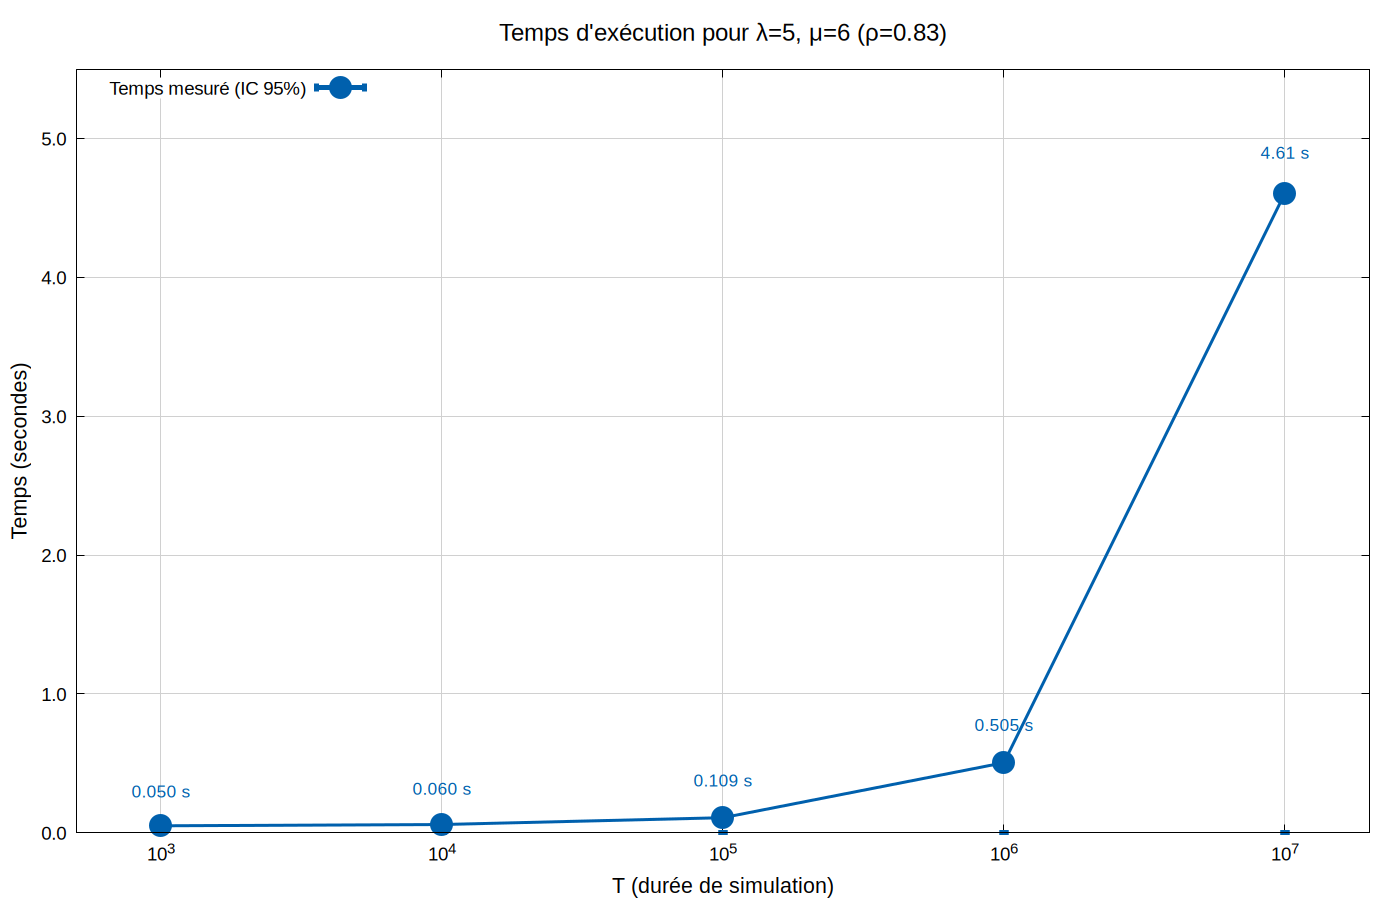
\includegraphics[width=0.8\textwidth]{../graphes/execution_time_vs_n.png}
    \caption{Temps d'exécution en fonction de la durée de simulation T (avec $\lambda=5$, $\mu=6$)}
    \label{fig:exec_time}
\end{figure}

\textbf{Observations} :

\begin{itemize}
    \item \textbf{Croissance accélérée} : La courbe montre une croissance légère et presque linéaire entre $10^3$ et $10^5$, puis une nette accélération entre $10^5$ et $10^6$ et enfin une croissance d'autant plus élevée entre $10^6$ et $10^7$ révélant l'impact de l'accumulation d'événements dans l'échéancier. Le nombre d'événements est proportionnel à T ($(\lambda + \mu) \times T$).
    
    \item \textbf{Performance} : Le temps d'exécution maximal moyen est de 4.61s pour T=$10^7$, ce qui est dans l'ordre de grandeur attendu pour une simulation de 50 millions de clients.
    
    \item \textbf{Impact des structures de données} : Pour les petites durées, les surcoûts d'initialisation dominent. Au-delà de $10^5$, le coût d'insertion dans l'échéancier croît avec sa taille, expliquant l'accélération observée.
\end{itemize}

\begin{figure}[H]
    \centering
    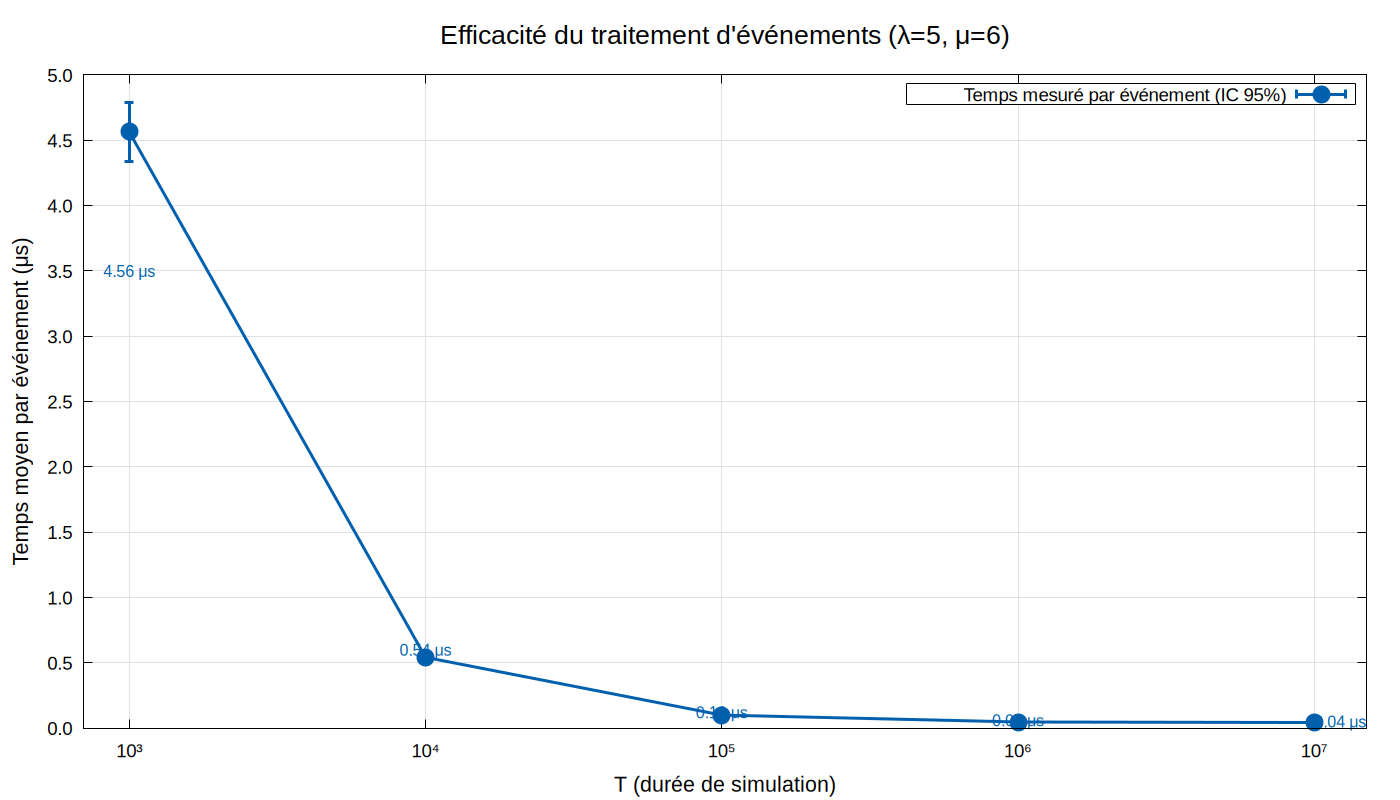
\includegraphics[width=0.8\textwidth]{../graphes/time_per_event.png}
    \caption{Temps moyen de traitement par événement}
    \label{fig:time_per_event}
\end{figure}

\textbf{Analyse du temps par événement} :

La \hyperref[fig:time_per_event]{Figure 10} montre la décroissance du temps moyen de traitement par événement en fonction de la durée de simulation T, avec les intervalles de confiance à 95\%.

\begin{itemize}
    \item \textbf{Décroissance rapide} : Le temps par événement chute de 4.6 $\mu$s à $10^3$ jusqu'à 0.04 $\mu$s à $10^7$.
    
    \item \textbf{Convergence asymptotique} : Pour T $\geq 10^6$, le temps par événement converge vers 0.04-0.05 $\mu$s, démontrant que les optimisations (tableau de recyclage, insertion efficace) sont efficaces pour les grandes simulations.  
    
    \item \textbf{Interprétation} : Cette décroissance s'explique par l'amortissement des coûts d'initialisation sur un nombre croissant d'événements. Pour T=$10^3$, on traite environ 11\,000 événements ; pour T=$10^7$, on traite environ 110 millions d'événements, soit un coût unitaire beaucoup plus faible grâce à l'amortissement des surcoûts d'initialisation.
    
    \item \textbf{Note sur les intervalles de confiance} : Les IC sont relativement plus grands pour T petit (T=$10^3$ : ±5\%) car on a moins d'événements et donc moins de données statistiques.
\end{itemize}

\subsubsection{Impact du taux d'arrivée \texorpdfstring{$\lda$}{lambda}}

Nous avons également étudié l'impact du taux d'arrivée $\lambda$ sur le temps d'exécution pour une durée fixe T, comme illustré dans la \hyperref[fig:exec_time_lambda]{Figure 11}.

\begin{figure}[H]
    \centering
    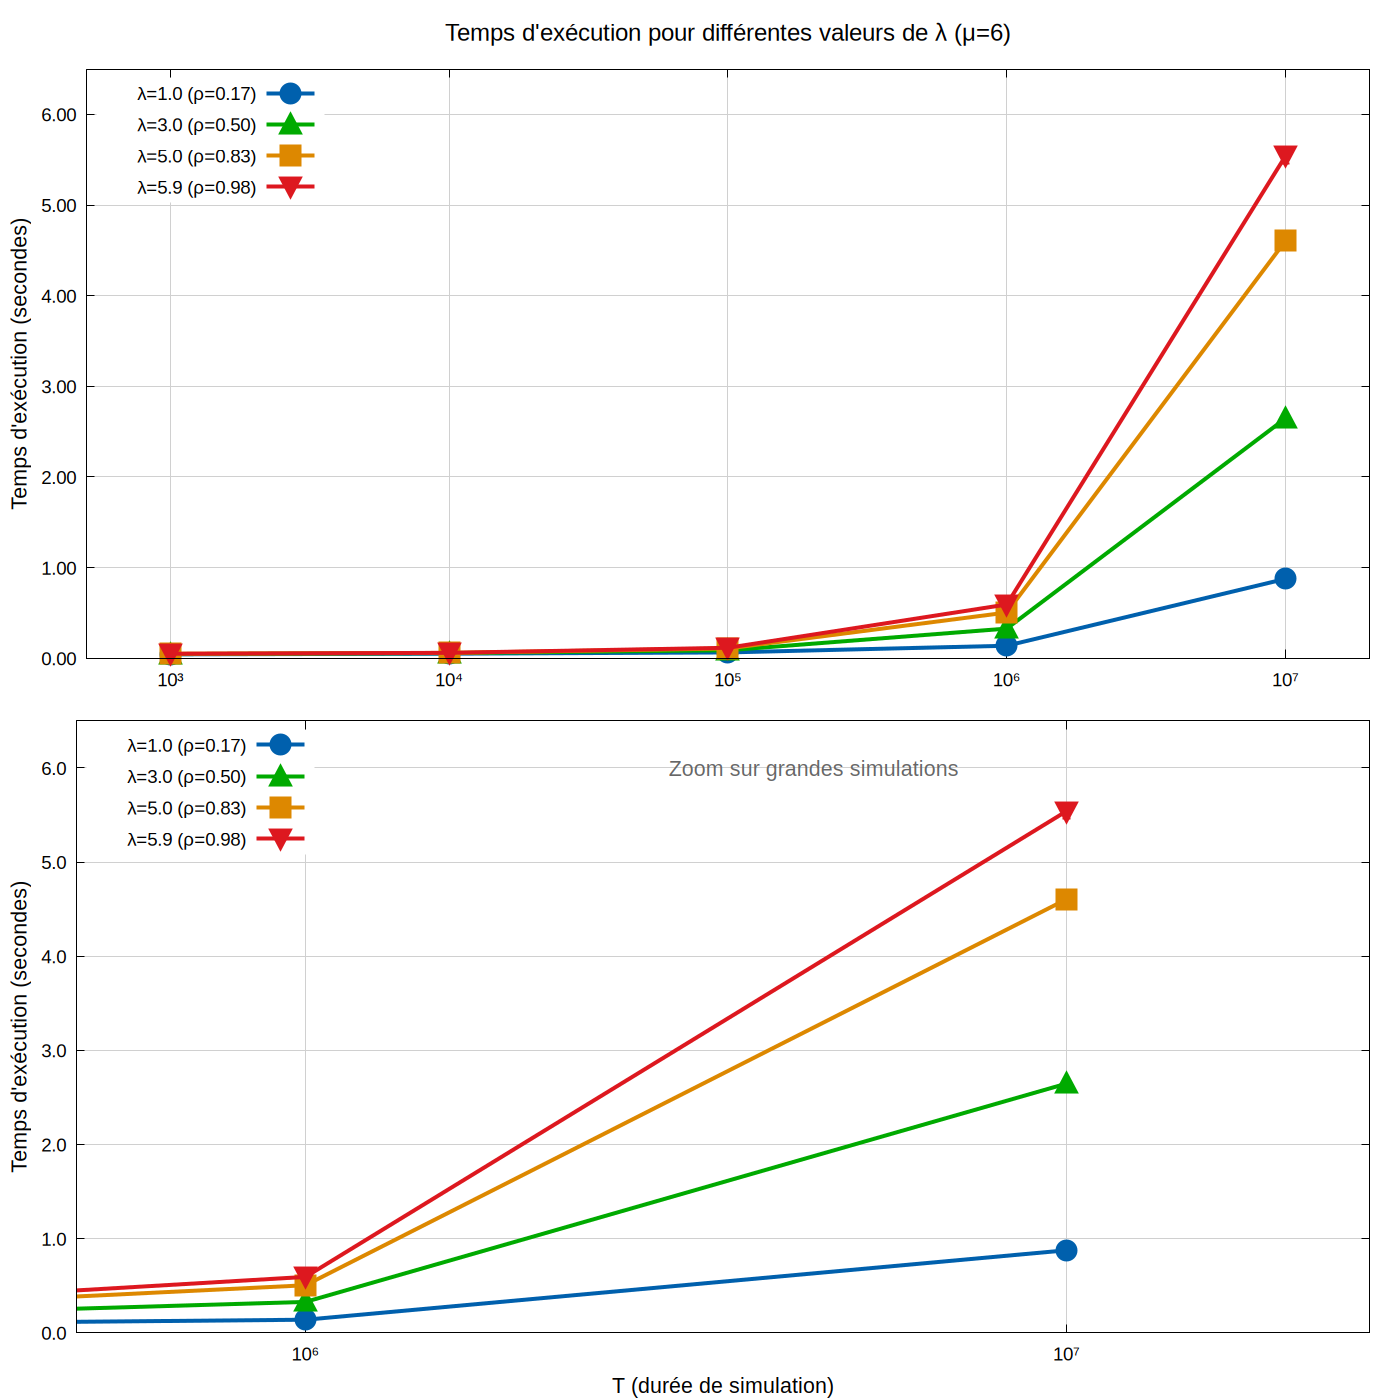
\includegraphics[width=0.8\textwidth]{../graphes/execution_time_lambda_comparison.png}
    \caption{Temps d'exécution pour différentes valeurs de $\lambda$ (durée fixe)}
    \label{fig:exec_time_lambda}
\end{figure}

\textbf{Observations} :

La \hyperref[fig:exec_time_lambda]{Figure 11} compare l'impact du taux d'arrivée $\lambda$ sur les temps d'exécution. Le panel supérieur offre une vue d'ensemble sur toutes les durées, tandis que le panel inférieur zoome sur les grandes simulations.

\begin{itemize}
    \item \textbf{Hiérarchie des temps d'exécution} : Les courbes montrent une nette hiérarchie croissante avec $\lambda$ : les valeurs faibles ($\lambda=1.0$, $\ro=0.17$) génèrent les temps les plus courts, tandis que les valeurs élevées ($\lambda=5.9$, $\ro=0.98$) produisent les temps les plus longs. Cette relation s'explique par le nombre d'événements $(\lambda + \mu) \times T$.
    
    \item \textbf{Croissance accélérée avec la durée} : Le panel supérieur révèle une croissance progressive puis accélérée pour toutes les valeurs de $\lambda$. Les petites durées montrent des courbes proches, tandis que les grandes durées (T $\geq 10^6$) révèlent une forte divergence entre les courbes, confirmant l'impact croissant de $\lambda$ sur les performances.
    
    \item \textbf{Augmentation de l'écart entre les courbes} : Le panel inférieur (zoom) illustre particulièrement bien l'effet : l'écart entre les différentes valeurs de $\lambda$ s'accentue significativement entre T=$10^6$ et T=$10^7$, révélant que plus $\lambda$ se rapproche de $\mu$, plus la complexité du système augmente.
    
    \item \textbf{Précision statistique} : Les intervalles de confiance (IC à 95\%) sont calculés mais pas nécessairement visibles sur les deux panels à cause des échelles différentes et les intervalles assez petits pour ne pas être visibles.
\end{itemize}

\subsection{Conclusion et interprétation croisée}

Cette analyse des performances révèle plusieurs aspects complémentaires du simulateur :

\vspace{0.3cm}
\textbf{Complexité temporelle et rôle des paramètres :} L'analyse croisée des \hyperref[fig:exec_time]{Figures 9}-\hyperref[fig:time_per_event]{10}-\hyperref[fig:exec_time_lambda]{11} confirme que le temps d'exécution croît essentiellement avec la durée de simulation T et le taux d'arrivée $\lambda$. Les optimisations (recyclage d'événements, insertion efficace dans l'échéancier) permettent de maintenir une complexité proche de O(N) même pour de très grandes simulations, mais l'accumulation d'événements dans l'échéancier induit une croissance non linéaire pour les très grandes durées (T $\geq 10^6$).

\vspace{0.3cm}
\textbf{Performance en fonction de $\lambda$ :} L'impact de $\lambda$ sur les temps d'exécution révèle un effet croissant avec la durée. Pour T $\geq 10^6$, l'écart entre les différentes valeurs de $\lambda$ s'amplifie significativement, confirmant que plus le facteur d'utilisation s'approche de 1, plus la complexité de gestion de l'échéancier augmente. Cet effet est particulièrement visible dans le panel zoom de la \hyperref[fig:exec_time_lambda]{Figure 11}.

\vspace{0.3cm}
\textbf{Limites pratiques :} Malgré les optimisations, les simulations avec T $\geq 10^8$ provoquent des erreurs de mémoire (\texttt{OutOfMemoryError}) dues à l'accumulation d'événements dans l'échéancier et au stockage des temps d'arrivée. Cette limite suggère que pour des simulations extrêmement longues, une approche différente serait nécessaire.

\vspace{0.3cm}
\textbf{Efficacité des optimisations :} Les \hyperref[fig:exec_time]{Figures 9}-\hyperref[fig:time_per_event]{10} montrent que le temps par événement converge vers une valeur très faible (0.04-0.05 $\mu$s pour T $\geq 10^6$), démontrant l'efficacité des structures optimisées à grande échelle. Les surcoûts d'initialisation dominent pour les petites simulations, mais deviennent négligeables avec l'augmentation de la durée.

%=============================================================================
% SYNTHÈSE ET RÉFLEXIONS
%=============================================================================

\section{Synthèse et Réflexions}

\subsection{Résultats et contributions}

Cette étude a permis de confirmer les propriétés théoriques des files M/M/1 par simulation discrète. Les résultats montrent une excellente correspondance entre simulation et théorie pour toutes les métriques, avec des erreurs relatives inférieures à 0.1\% sur toute la plage de $\rho$. Les intervalles de confiance étroits valident la robustesse statistique du simulateur. Les analyses de sensibilité révèlent que les instabilités observées près de la saturation sont des propriétés mathématiques fondamentales du modèle M/M/1, confirmées par l'analyse théorique des dérivées partielles de $L$ et $W$ par rapport à $\rho$, qui divergent lorsque $\rho \to 1$.

Les performances obtenues sont satisfaisantes et dans la plage attendue. Les optimisations implémentées (recyclage d'événements, insertion efficace dans l'échéancier) ont permis d'atteindre une complexité proche de O(N), avec un temps par événement convergeant vers 0.04-0.05 $\mu$s pour les grandes simulations. Cependant, l'accumulation d'événements dans l'échéancier induit une croissance non linéaire pour les grandes durées, et les simulations très longues (T $\geq 10^8$) provoquent des erreurs de mémoire (\texttt{OutOfMemoryError}).

\subsection{Améliorations possibles}

Plusieurs améliorations pourraient être envisagées au niveau de l'implémentation :

\begin{itemize}
    \item \textbf{Structure de données optimisée} :\newline Remplacer la \texttt{LinkedList} par une \texttt{PriorityQueue} (tas binaire) permettrait d'avoir un coût d'insertion en O(log n) garantie au lieu de O(n) dans le pire cas pour la LinkedList, même si l'optimisation actuelle amortit à O(1) pour les insertions en fin de liste.
    
    \item \textbf{Gestion mémoire pour simulations longues} : Implémenter un mécanisme de vidage périodique de l'échéancier ou limiter sa taille maximale pour éviter les erreurs \texttt{OutOfMemoryError}.
    
    \item \textbf{Optimisations du tableau de recyclage} : Redimensionner dynamiquement le tableau de recyclage avec croissance exponentielle pour éviter la limitation de taille fixe (TAILLE\_MAX\_RECYCLAGE=10000).

\end{itemize}

\subsection{Apprentissages}

Cette implémentation a permis de comprendre que la gestion de l'échéancier est critique pour les performances, et que la validation statistique (IC, rejeux) est essentielle pour garantir la robustesse des résultats. Le compromis entre précision et temps de calcul nécessite un arbitrage : simulations longues pour la précision vs optimisations pour les performances.

\subsection{Limitations du modèle M/M/1}

L'analyse révèle trois catégories de limitations. \textbf{Mathématiques} : Le modèle explose lorsque $\rho \to 1$, avec un seuil critique $\rho=0.9$ rendant le système inutilisable. \textbf{Simulateur} : Les erreurs mémoire apparaissent pour T $\geq 10^8$, et la précision statistique se dégrade fortement pour $\rho > 0.9$ avec une croissance non linéaire des coûts de gestion. \textbf{Systèmes réels} : Les hypothèses de capacité infinie, processus Poisson et service exponentiel simplifient excessivement la réalité, excluant la priorisation et les abandons. Le modèle M/M/1 reste adapté pour $\rho < 0.8$, garantissant qualité de service, temps d'attente raisonnables et précision statistique fiable.
\end{document}

